% 原文 pp.107–114（印刷 pp.1225–1232）
\section{Lecture 8：Abel 对偶}

\begin{keytakeaways}
本讲系统讲述二维、三维、四维中的 Abel 对偶（abelian duality）：把取值于圆周 $S^1$ 的标量场（或 $U(1)$ 联络）与另一套自由度互换，使强弱耦合对调。二维情形是半径 $R$ 的圆周上的自由场与半径 $1/R$ 的自由场之间的等价（「$R$ 变成 $1/R$」），推导只用一个 Lagrange 乘子场 $\sigma$ 与 Gauss 积分，却给出配分函数之间的精确关系，其中含与 Euler 示性数有关的因子 $(R/2\pi)^{\chi(\Sigma)}$；同一框架下算符 $d\phi$ 对偶到 $-\frac{i}{R^2}\ast d\sigma$，而顶点算符 $e^{in\phi(P)}$ 对偶到「删去该点、并对具有给定缠绕数的 $\sigma$ 求和」这一非局部处方。三维情形把 $S^1$ 值标量场对偶到规范耦合 $e=\sqrt{\Lambda}$ 的 $U(1)$ 规范场，从而把 Laplace 方程的解与 Maxwell 方程的解对应起来，并把 $e^{in\phi(P)}$ 对应到「在 $P$ 附近第一 Chern 类为 $n$ 的线丛上求和」，这是磁单极子算符的雏形；四维情形则与 $SL(2,\mathbb{Z})$ 有关，将在 Donaldson 理论中使用。作为应用，本讲末尾以三维对偶讨论 Polyakov 的 $SO(3)$ 规范-Higgs 模型，给出二维以上关于禁闭（confinement）现象最具体的可解模型之一。
\end{keytakeaways}

% ===== 原文 p.107 =====
\subsection{引言}
% 原文 §8.1：Introduction

今天，我们将讨论二维、三维与四维中的 Abel 对偶。

在二维，Abel 对偶把圆的半径 $R$ 反演，通常被称为「$R$ 变成 $1/R$」的等价。在某个超对称（supersymmetry）版本中，它导致镜像对称（mirror symmetry）的一个线性版本。

在三维，研究完对偶之后，我们将给出它在 Polyakov 的禁闭（confinement）模型中的一个应用。

四维的 Abel 对偶与一个 $SL(2,\mathbb{Z})$ 对称性有关，我们最终会用它来理解 Donaldson 理论，也就是四维的 $\mathcal{N}=2$ 超对称理论。在此过程中我们会找到另一个禁闭模型。事实上，对偶的这两个应用给出了二维以上已知的、关于禁闭现象的最具体的模型。

我们首先给出对偶的经典表述。在二维，考虑一个含有场 $\phi$、$\sigma$ 的理论，二者都满足 Laplace 方程
\begin{equation}
  \tag{8.1}
  \label{eq:8-1}
  \nabla^2\phi=0;\qquad \nabla^2\sigma=0,
\end{equation}
并通过
\begin{equation}
  \tag{8.2}
  \label{eq:8-2}
  d\phi=\ast d\sigma
\end{equation}
相联系。经典地，这两个场中的任何一个都可以取作该理论的基本场。例如，若我们从满足 $\nabla^2\sigma=\ast d\ast d\sigma=0$ 的 $\sigma$ 出发，则 $d\ast d\sigma=0$，于是局部地可以写下 $\ast d\sigma=d\phi$，其中 $\phi$ 是某个场；也就是说，$\sigma$ 决定了 $\phi$（局部地，且差一个可加常数）。

% [Tutor Note: (8.2) 与四维的 (8.5) 在几何上并不同类：二维欧氏空间中 Hodge 星作用于 1-形式满足 $\ast^2=-1$，故 $d\phi=\ast d\sigma$ 等价于 $d\sigma=-\ast d\phi$，它其实是「闭且余闭的 1-形式局部必为某函数的微分」这一 Hodge 分解的表述，而非自对偶条件；只有在四维，$\ast^2=+1$ 作用于 2-形式，(8.5) $F_A=\ast F_B$ 才有把曲率劈为自对偶/反自对偶部分的意义（这正是 Donaldson 理论的入口）。若把二维的 $\ast^2=-1$ 误记为 $+1$，则 (8.17)→(8.19) 配平方时残留项的符号会整个反过来。]

同样地，在三维，考虑一个含场 $\phi$ 的理论，$\phi$ 满足 Laplace 方程；再考虑某个线丛（line bundle）$\mathcal{L}$ 上的联络 $A$，其曲率 $F=dA$ 满足 Maxwell 方程
\begin{equation}
  \tag{8.3}
  \label{eq:8-3}
  dF=d\ast F=0,
\end{equation}
其对偶关系为
\begin{equation}
  \tag{8.4}
  \label{eq:8-4}
  \ast d\phi=F.
\end{equation}
再次同上，这两个场中的任何一个都可以取作基本场。

% [Tutor Note: (8.3)–(8.4) 的实质是「交换 Bianchi 恒等式与场方程」：给定 $\phi$ 调和，令 $F=\ast d\phi$，则 $dF=dd\phi=0$ 自动成立，而 $d\ast F=\pm d\ast\ast d\phi=\pm dd\phi=0$（三维中 2-形式上 $\ast^2=+1$）；反之，由 $dF=d\ast F=0$ 知 $\ast F$ 闭且余闭，故局部等于 $d\phi$。注意 $F=dA$ 只在 $\mathcal{L}$ 平凡时整体成立，否则 $F$ 只是 $\mathcal{L}$ 的曲率，$\frac{1}{2\pi}\int F$ 为整数（第一 Chern 类）——这一整体性在三维对偶中正是磁单极子荷的来源，参见 (8.30) 之后关于 $H^1(M,\mathbb{R}/\mathbb{Z})$ 的讨论。]

\noindent\textit{（本讲笔记由 David Morrison 整理。）}

% ===== 原文 p.108 =====
在四维，类似物是线丛 $\mathcal{L}_A$ 与 $\mathcal{L}_B$ 上的两个联络 $A$ 与 $B$，二者各自满足 Maxwell 方程，并通过
\begin{equation}
  \tag{8.5}
  \label{eq:8-5}
  F_A=\ast F_B
\end{equation}
相联系。

就 Abel 对偶而言，只要愿意，我们还可以继续走向更高维；但要找到有趣的应用，就得进入弦论。

\subsection{二维对偶}
% 原文 §8.2：Duality in two dimensions

我们想研究这些经典陈述的量子版本。先从二维情形开始。我们把 $S^1$ 等同于 $\mathbb{R}/2\pi\mathbb{Z}$，并在圆上使用加法坐标。取 $\phi$ 为映射 $\phi:\Sigma\to S^1$，其中 $\Sigma$ 是紧致可定向曲面，配有 Riemann 度量 $g_{\alpha\beta}$。（稍后我们会考虑一个变体：在其中 $\phi$ 不要求在若干指定点 $P_i$ 处有定义，也就是说，$\phi$ 将把 $\Sigma-\{P_i\}$ 映入 $S^1$。）我们的拉格朗日量\footnote{本讲所有拉格朗日量都写在欧氏号差（Euclidean signature）下。}为
\begin{equation}
  \tag{8.6}
  \label{eq:8-6}
  \mathcal{L}(\phi)=\frac{R^2}{4\pi}\int d^2x\,\sqrt{g}\,\partial_\alpha\phi\,\partial^\alpha\phi
  =\frac{R^2}{4\pi}\int d\phi\wedge\ast d\phi .
\end{equation}
其运动方程 $dd\phi=d\ast d\phi=0$ 再现了上面讨论的经典理论。

% [Tutor Note: (8.6) 的系数并非任意。把靶空间取为半径 $R$ 的圆、令 $\phi$ 的周期为 $2\pi$，则靶空间度量为 $R^2d\phi^2$，于是 $\mathcal{L}=\frac{R^2}{4\pi}(\partial\phi)^2$ 正是「半径 $R$ 的圆」上的自由场；等价地，令 $\phi=y/R$（$y$ 的周期为 $2\pi R$）即得标准的 $\frac{1}{4\pi}(\partial y)^2$。这也解释了为何对偶理论 (8.21) 的耦合是 $1/R^2$：对偶把靶空间度量取倒数。若把 (8.6) 的 $R^2$ 误当作「$1/g^2$」式的规范耦合，就会把 $R\to1/R$ 误解为一个平凡的重命名，而看不到它交换了「动量模」与「缠绕模」。]

我们将用多种方式研究这个理论。惯用的技巧是：引入新变量，使得把它们积掉（integrate out）会回到原来的理论；然后反过来把旧变量积掉而保留新变量，以便得到该理论的对偶表述。

所以我们实际上要研究另一个理论，它含有场 $\phi$ 与 $A$，其中 $\phi$ 是平凡 $S^1$-丛 $\mathcal{S}$ 的一个截面，$A$ 是 $\mathcal{S}$ 上的一个联络。选取 $\mathcal{S}$ 的一个平凡化 $\phi_0$（于是 $A=\phi_0^\ast\tilde A$，其中 $\tilde A$ 是丛的全空间上的某个 1-形式），我们可以定义协变导数
\begin{equation}
  \tag{8.7}
  \label{eq:8-7}
  D_A\phi=d\phi+A,
\end{equation}
并引入新的拉格朗日量
\begin{equation}
  \tag{8.8}
  \label{eq:8-8}
  \mathcal{L}(\phi,A)=\frac{R^2}{4\pi}\int d^2x\,\sqrt{g}\,(\partial_\alpha\phi+A_\alpha)(\partial^\alpha\phi+A^\alpha)
  =\frac{R^2}{4\pi}\int D_A\phi\wedge\ast D_A\phi .
\end{equation}
虽然令 $A$ 为零即可回到旧的拉格朗日量，但并没有任何机制强制这一点，除非我们再引入第三个场 $\sigma$，让它扮演 Lagrange 乘子（Lagrange multiplier）的角色。我们取 $\sigma$ 为从 $\Sigma$ 到 $S^1$ 的映射，并写下拉格朗日量
\begin{equation}
  \tag{8.9}
  \label{eq:8-9}
  \mathcal{L}(\phi,A,\sigma)=\frac{R^2}{4\pi}\int D_A\phi\wedge\ast D_A\phi-\frac{i}{2\pi}\int\sigma\wedge F_A,
\end{equation}
其中 $F_A$ 是 $A$ 的曲率。

最后这一项需要作些说明。由于我们假定圆丛 $\mathcal{S}$ 是平凡的，可以整体地写出 $F_A=dA$，而最后一项应被理解为 $\frac{i}{2\pi}\int d\sigma\wedge A$（在分部积分之后）；之所以需要这一步，是因为 $\sigma$ 不是单值的。更一般地，即使 $\mathcal{S}$ 非平凡，也可以用一点拓扑来定义这样的项，即定义 $\exp\bigl(\frac{i}{2\pi}\int\sigma\wedge F_A\bigr)$，其做法类似于定义 Chern–Simons 形式。

写下这个拉格朗日量的要点在于：$\mathcal{L}(\phi,A,\sigma)$ 等价于 $\mathcal{L}(\phi)$，下面我们就来证明。一个朴素的分析如下：$\sigma$ 不出现在任何导数中，

% ===== 原文 p.109 =====
而它的运动方程是 $F_A=0$；施加这一条件后，我们就可以走到一个 $A=0$ 的规范，从而回到原来的理论。

更整体地，我们考虑路径积分
\begin{equation}
  \tag{8.10}
  \label{eq:8-10}
  Z=\frac{1}{\mathrm{vol}(G)}\int\mathcal{D}\phi\,\mathcal{D}A\,\mathcal{D}\sigma\,
  \exp\Bigl[-\frac{R^2}{4\pi}\int D_A\phi\wedge\ast D_A\phi+\frac{i}{2\pi}\int\sigma\wedge F_A\Bigr].
\end{equation}
（眼下我们先关注配分函数，但带算符插入的路径积分也可以用同样的方式处理，这一点我们稍后再讨论。）借助标准公式
\begin{equation}
  \tag{8.11}
  \label{eq:8-11}
  \int\frac{dx}{2\pi}\,e^{ixy}=\delta(y),
\end{equation}
我们想说：做完 $\sigma$ 积分就会把 $F_A$ 置零。对这一断言应当谨慎，因为我们研究的是取值于圆周的函数。

% [Tutor Note: (8.11) 只是 $\mathbb{R}$ 上的 $\delta$ 函数表示；而这里 $\sigma$ 取值于圆群 $S^1$，$\int\mathcal{D}\sigma\,e^{\frac{i}{2\pi}\int\sigma\wedge F_A}$ 实际上不是 $\delta(F_A)$，而是「按缠绕数分层求和」之后的 $\delta$ 函数梳——这正是 (8.12) 要写出的内容。换言之 (8.11) 的等式与 (8.10) 之间差着一次对 $d\sigma_h\in H^1(\Sigma,2\pi\mathbb{Z})$ 的求和；若直接把 (8.11) 用在圆值场上，会漏掉 (8.13) 中整个 $\prod_j\sum_{m_j}$ 因子，也就得不到 (8.15) 里第二个 $\delta$ 函数。]

记住我们把 $S^1$ 等同于 $\mathbb{R}/2\pi\mathbb{Z}$，映射 $\sigma:\Sigma\to S^1$ 局部上可以写成一个实值函数，但它未必整体单值；不过 $d\sigma$ 将是 $\Sigma$ 上（单值的）实 1-形式。选取圆周值函数 $\sigma_h:\Sigma\to S^1$，使 $d\sigma_h$ 是 $d\sigma$ 的 de Rham 上同调类中的调和代表元（harmonic representative）。（我们这样规范 $\sigma_h$ 的选取：取定某点 $P\in\Sigma$，并要求 $\sigma_h(P)\in2\pi\mathbb{Z}$。）于是可以写 $\sigma=\sigma_h+\sigma_{\mathbb{R}}$，其中 $\sigma_{\mathbb{R}}$ 是单值实函数。

注意 $\frac{1}{2\pi}d\sigma$，等价地 $\frac{1}{2\pi}d\sigma_h$，必须有整周期。特别地，若取整系数调和 1-形式的一组基 $\lambda_j$，并写 $d\sigma_h=\sum2\pi m_j\lambda_j$，则 $m_j\in\mathbb{Z}$。

现在来计算：
\begin{align}
  \tag{8.12}
  \label{eq:8-12}
  \int\mathcal{D}\sigma\,e^{\frac{i}{2\pi}\int\sigma\wedge F_A}
  &=\int\mathcal{D}\sigma_{\mathbb{R}}\,e^{\frac{i}{2\pi}\int\sigma_{\mathbb{R}}\wedge F_A}
  \sum_{d\sigma_h\in H^1(\Sigma,2\pi\mathbb{Z})}e^{-\frac{i}{2\pi}\int d\sigma_h\wedge A}\\
  \tag{8.13}
  \label{eq:8-13}
  &=\delta(F_A)\prod_j\Bigl(\sum_{m_j\in\mathbb{Z}}e^{-im_j\int\lambda_j\wedge A}\Bigr).
\end{align}

第一个因子告诉我们 $A$ 是平坦联络（flat connection）。此外，在平坦联络之中，规范等价类 $[A]$ 由和乐（holonomy）标记，等价地由量 $\int\lambda_j\wedge A$ 标记。由于被积函数的其余部分规范不变，我们可以规范固定（略去因子 $(\mathrm{vol}(G))^{-1}$），并在规范等价类的空间上积分（这是一个有限维积分）：
\begin{align}
  \tag{8.14}
  \label{eq:8-14}
  Z&=\int\mathcal{D}\phi\,\mathcal{D}[A]\,e^{-\frac{R^2}{4\pi}\int D_A\phi\wedge\ast D_A\phi}\delta(F_A)
  \prod_j\Bigl(\sum_{m_j\in\mathbb{Z}}e^{-im_j\int\lambda_j\wedge A}\Bigr)\\
  \tag{8.15}
  \label{eq:8-15}
  &=\int\mathcal{D}\phi\,e^{-\frac{R^2}{4\pi}\int D_A\phi\wedge\ast D_A\phi}\delta(F_A)\,
  \delta\Bigl(\int\lambda_i\wedge A=0\quad\mathrm{mod}\ 2\pi\mathbb{Z}\Bigr).
\end{align}

% [Tutor Note: (8.12)→(8.13) 是格上的 Poisson 求和（等价于圆群上的 Fourier 变换）：对缠绕数分层求和后，$\int\mathcal{D}\sigma_{\mathbb{R}}$ 给出 $\delta(F_A)$，而对 $d\sigma_h$ 的和给出环面 $H^1(\Sigma,\mathbb{R})/H^1(\Sigma,2\pi\mathbb{Z})$ 上的 $\delta$ 函数梳，即 (8.15) 中第二个 $\delta$。作者只说「现在来计算」。技术上有两点须留意：其一，$\lambda_j$ 必须是整系数调和 1-形式的基（使 $\int_\Sigma\lambda_i\wedge\lambda_j$ 为交截数矩阵），否则「周期为 $2\pi$ 的整数倍」无从谈起；其二，$\sum_{m_j\in\mathbb{Z}}e^{-im_j\int\lambda_j\wedge A}$ 在 $\int\lambda_j\wedge A\equiv0\ (2\pi)$ 处发散，故它只在该超曲面上有支撑，写成一个 $\delta$ 是形式上的简写。]

于是出现了把和乐与曲率同时置零的 $\delta$ 函数。所以 $A$ 在模规范变换的意义下为零，而我们这个新理论确实等价于原来的理论，其配分函数为
\begin{equation}
  \tag{8.16}
  \label{eq:8-16}
  Z=\int\mathcal{D}\phi\,\exp\Bigl(-\frac{R^2}{4\pi}\int d\phi\wedge\ast d\phi\Bigr).
\end{equation}

现在让我们以相反的次序积分，即积掉 $\phi$ 与 $A$ 而保留 $\sigma$。为积掉 $\phi$，我们这样规范固定：使 $\phi=0$，

% ===== 原文 p.110 =====
并从而在路径积分中略去因子 $(\mathrm{vol}(G))^{-1}$。于是路径积分 (8.10) 约化为
\begin{equation}
  \tag{8.17}
  \label{eq:8-17}
  \int\mathcal{D}A\,\mathcal{D}\sigma\,\exp\Bigl[-\frac{R^2}{4\pi}\int A\wedge\ast A+\frac{i}{2\pi}\int\sigma\wedge F_A\Bigr].
\end{equation}
你也许会乐于验证：与这一规范固定相应的 Faddeev–Popov 行列式是
\begin{equation}
  \tag{8.18}
  \label{eq:8-18}
  \int\mathcal{D}c\,\mathcal{D}\bar c\,\exp\Bigl[-\frac{R^2}{4\pi}\int d^2x\,\bar c\,c\Bigr].
\end{equation}

% [Tutor Note: 规范固定 $\phi=0$（即把 $\phi\to\phi+\epsilon$ 的平移对称固定掉）给出的 Faddeev–Popov 算符是 $d:\Omega^0\to\Omega^1$，其行列式为 $(\det\Delta_0)^{1/2}$。作者把它写成 $\int\mathcal{D}c\,\mathcal{D}\bar c\,e^{-\frac{R^2}{4\pi}\int\bar cc}$，并在脚注 2 中特意声明「把 $c$ 看作 0-形式、$\bar c$ 看作 2-形式」：这不是文字游戏，而是因为二维 Hodge 分解给出 $\det\Delta_1=\det\Delta_0\det\Delta_2$（略去调和模），只有按 $0$-形式与 $2$-形式（各 $n_0=n_2$ 个模）来计数，鬼场因子才能与下面 $A'$ 的高斯积分逐项配对，从而产生 (8.20) 中的指数 $(-n_0+n_1-n_2)$。]

为对 $A$ 积分，我们需要配方（complete the square），把指数中的第二项看作 $-\frac{i}{2\pi}\int A\wedge d\sigma$，也就是说，它是 $A$ 的线性项。我们作变量替换 $A'=A+\frac{i}{R^2}\ast d\sigma$；结果（包含 Faddeev–Popov 积分）为
\begin{equation}
  \tag{8.19}
  \label{eq:8-19}
  \Bigl(\int\mathcal{D}c\,\mathcal{D}\bar c\,e^{-\frac{R^2}{4\pi}\int d^2x\,\bar c\,c}\Bigr)
  \Bigl(\int\mathcal{D}A'\,e^{-\frac{R^2}{4\pi}\int A'\wedge\ast A'}\Bigr)
  \Bigl(\int\mathcal{D}\sigma\,e^{-\frac{1}{4\pi R^2}\int d\sigma\wedge\ast d\sigma}\Bigr).
\end{equation}
（对 $A'$ 的 Gauss 积分，如同 Faddeev–Popov 行列式，可以看作归一化因子。）

% [Tutor Note: 这一步的平移是「虚平移」：$A'=A+\frac{i}{R^2}\ast d\sigma$ 中的 $i$ 意味着 $A$ 被解析延拓为复值联络，否则线性项 $-\frac{i}{2\pi}\int A\wedge d\sigma$ 不能被实平移消掉。按标准 Gauss 积分 $\int dA\,e^{-aA^2+bA}\propto e^{b^2/4a}$ 逐项验算：$a=\frac{R^2}{4\pi}$、$b=-\frac{i}{2\pi}$（线性项耦合的是 $\ast d\sigma$，而 $A\wedge\ast(\ast d\sigma)=-A\wedge d\sigma$ 用到二维 1-形式上 $\ast\ast=-1$），于是 $b^2/4a=+\frac{1}{4\pi R^2}$。若把 $A$ 当作实场，残留项就是正的，对偶理论看似发散；而 (8.19) 给出的负号只能来自 $A$ 积分轮廓的转动（等价于 $A\to iA$），即作者写下 (8.17) 时已默认联络复化。取使对偶作用量负定、积分收敛的那一支，与 (8.21) 的最终结果自洽。符号若不追到轮廓这一步，最容易得出「对偶理论发散」的错误结论。]

Faddeev–Popov 积分对 $\Sigma$ 上每个 0-形式与每个 2-形式各给出一个因子 $\bigl(\int dt\,e^{-tR^2/4\pi}\bigr)^{-1}$\footnote{为此，请把 $c$ 看作一个 0-形式、把 $\bar c$ 看作一个 2-形式。}；对 $A'$ 的积分对 $\Sigma$ 上每个 1-形式给出一个因子 $\int dt\,e^{-tR^2/4\pi}$。于是，若以 $n_j$ 记「$\Sigma$ 上 $j$-形式的个数」，这些项合起来给出总的因子
\begin{equation}
  \tag{8.20}
  \label{eq:8-20}
  \bigl(\sqrt{\pi}/(R^2/4\pi)\bigr)^{(-n_0+n_1-n_2)}=(R/2\pi)^{\chi(\Sigma)}.
\end{equation}

% [Tutor Note: 这里 (8.20) 左右两端按字面并不相等，是原书的一处笔误：以 $a=R^2/4\pi$ 记之，$\int dt\,e^{-ta}=\sqrt{\pi/a}$，故每个 0-形式与 2-形式贡献 $(\sqrt{\pi/a})^{-1}$、每个 1-形式贡献 $(\sqrt{\pi/a})^{+1}$，总因子应为 $\bigl(\sqrt{\pi}/\sqrt{R^2/4\pi}\bigr)^{(-n_0+n_1-n_2)}=(2\pi/R)^{(-n_0+n_1-n_2)}$；再用 $\chi(\Sigma)=2-2g=n_0-n_1+n_2$ 即得右端的 $(R/2\pi)^{\chi(\Sigma)}$。原书分母上的根号漏掉了（或等价地指数应减半），若照抄则两端相差 $(R/2\pi)^{2\chi}$。此处照原样译出，读者引用时请以右端为准。]

也就是说，联系这两个对偶表述的变换规则是
\begin{equation}
  \tag{8.21}
  \label{eq:8-21}
  \int\mathcal{D}\phi\,\exp\Bigl[-\frac{R^2}{4\pi}\int d\phi\wedge\ast d\phi\Bigr]
  =(R/2\pi)^{\chi(\Sigma)}\int\mathcal{D}\sigma\,\exp\Bigl[-\frac{1}{4\pi R^2}\int d\sigma\wedge\ast d\sigma\Bigr].
\end{equation}
（因子 $(R/2\pi)^{\chi(\Sigma)}$ 没有出现在今年其他讲者所作的具体计算中，因为他们的计算是在亏格 1 的情形做的。）第一个理论中的耦合 $R$ 映到第二个理论中的耦合 $1/R$，这就是为什么这个对偶有时被称为「$R$ 变成 $1/R$」。

% [Tutor Note: $(R/2\pi)^{\chi(\Sigma)}$ 是配分函数在 $R\to1/R$ 下的「反常」：$R$ 同时出现在作用量系数与测度归一化中，二者并不抵消。亏格 1 时 $\chi=0$、因子为 $1$，这正是作者说其他讲者在环面上的显式计算看不到它的原因；一般亏格下它必须用 $\zeta$ 函数正规化的行列式比值来定义，属于 $c=1$ 紧致玻色子的标准结果（可与 Polchinski 关于圆上玻色子 $T$-对偶的讨论对勘）。]

现在我们想追踪这个理论中的算符在对偶变换下的像，并确定它对关联函数以及配分函数的影响。一个容易的情形是 $d\phi$，我们预期它映到 $\ast d\sigma$，正如经典理论中那样（实际上，把归一化考虑进去后，它会映到 $\ast d\sigma$ 的一个倍数）。我们需要把上述计算重复一遍，但插入一些算符 $\prod_i\mathcal{O}_i(\phi)$，其中之一是 $d\phi$。为此，我们需要 $d\phi$ 的一个规范不变的扩充，而协变导数正好提供了它：
\begin{equation}
  \tag{8.22}
  \label{eq:8-22}
  d\phi(x)\ \bigl(\text{第一个理论}\bigr)\ \longrightarrow\ D_A\phi(x)\ \bigl(\text{大理论}\bigr).
\end{equation}
然后容易验证：当我们积掉 $\sigma$（并把 $A$ 规范固定为零）时，它映回 $d\phi$。

一般地，映射算符的困难之处在于：要为给定的算符找到它在更大的理论中的恰当扩充，

% ===== 原文 p.111 =====
而这个扩充在积掉 $\sigma$ 之后要回到原来的算符。对 $d\phi$ 来说这并不太难，正如我们刚刚看到的。

当路径积分中插入了 $D_A\phi$ 时，我们的计算会怎样改变？先前配方时，我们作了变量替换 $A'=A+\frac{i}{R^2}\ast d\sigma$。如果路径积分中已插入 $D_A\phi$，那么经过这一变量替换，它变为 $D_{A'}\phi-\frac{i}{R^2}\ast d\sigma$。在推导的其余部分，当 $\phi$ 被规范固定为零、$A'$ 被积掉之后，我们剩下的就是在对偶理论中插入 $-\frac{i}{R^2}\ast d\sigma$。因此，这就是 $d\phi$ 在对偶理论中的像。

在操作这些算符插入之间的映射时，必须小心。例如，尽管 $d\phi$ 映到 $-\frac{i}{R^2}\ast d\sigma$，但局部算符 $(d\phi)^2$ 在对偶理论中并不会映到 $\bigl(\frac{i}{R^2}\ast d\sigma\bigr)^2$，原因是在配方时引入了非线性。

% [Tutor Note: 这一段点出对偶的一个根本限制：只有「线性于导数」的算符有局部而简单的像。$d\phi\to D_A\phi$ 之所以干净，是因为 $D_A\phi=d\phi+A$ 与 $A$ 线性耦合，而 $A$ 的平移是常数平移；一旦算符含 $(D_A\phi)^2$，平移后会出现 $D_{A'}\phi$ 与 $\frac{i}{R^2}\ast d\sigma$ 的交叉项，它不与 $\sigma$ 解耦，于是像算符变成非局部的。等价地说，$R\to1/R$ 不是场空间之间的逐点映射，而是算符代数之间的同构，只在某些「顶点算符」上保持局部性——这正是下面要引入非局部对象 (8.23) 的动机。]

使这个情形容易的原因在于，协变导数是通常导数的一个自然的规范不变扩充。

更难对付的算符插入是 $e^{i\phi}$。它没有规范不变的版本。另一方面，我们其实并不需要它，因为 $\langle e^{i\phi(P)}\rangle=0$。但两点关联函数 $\langle e^{i\phi(P)}e^{-i\phi(Q)}\rangle$ 一般不为零，所以当 $P\ne Q$ 时，我们应当设法对这样的插入作对偶化。

我们要做一件相当奇怪的事。对这一对算符插入，不可能构造出局部的规范不变扩充；因此我们在对偶过程中（也就是说，在中间那个理论中）非局部地处理它，在路径积分中引入如下形式的项
\begin{equation}
  \tag{8.23}
  \label{eq:8-23}
  e^{i\phi(P)}e^{-i\phi(Q)}e^{\frac{i}{2\pi}\int\theta\wedge A},
\end{equation}
其中 $\theta$ 是 1-形式，满足
\begin{equation}
  \tag{8.24}
  \label{eq:8-24}
  \frac{1}{2\pi}d\theta=\delta_P-\delta_Q,
\end{equation}
且 $\theta$ 的所有周期在模 $2\pi\mathbb{Z}$ 的意义下为零。

% [Tutor Note: (8.24) 有解的前提是 $\delta_P-\delta_Q$ 作为分布是恰当形式，即 $P-Q$ 作为 0-链在 $H_0(\Sigma)$ 中为零；两个同次数的 0-链之差总是边缘，所以 $\theta$ 总存在——这就是「两点函数可以沿一条割线局域化」的拓扑根据。条件「所有周期 $\equiv0\ (2\pi\mathbb{Z})$」保证 $e^{\frac{i}{2\pi}\int\theta\wedge A}$ 不依赖于 $\theta$ 的选取；而 (8.25) 的规范不变性可直接验证：在 $A\to A+d\epsilon$ 下 $e^{i\int_\ell A}\to e^{i\int_\ell A}e^{i(\epsilon(Q)-\epsilon(P))}$，恰被 $e^{i\phi(P)}e^{-i\phi(Q)}$ 在 $\phi\to\phi-\epsilon$ 下的变换抵消。]

为找到这样的 $\theta$，取一条从 $P$ 到 $Q$ 的路径 $\ell$，并令 $\theta/2\pi$ 为 $\ell$ 的 Poincaré 对偶（把 $\ell$ 看作分布）。于是我们可以把我们的项 (8.23) 改写为
\begin{equation}
  \tag{8.25}
  \label{eq:8-25}
  e^{i\phi(P)}e^{i\int_\ell A}e^{-i\phi(Q)},
\end{equation}
这显然是规范不变的表达式。（这是 $\theta$ 的一种选法，但我们允许比这更一般的 $\theta'$。）最终我们会把 $\theta$ 看作 $\Sigma-P-Q$ 上平凡 $S^1$-丛上的一个联络形式。

这样，我们就找到了一个规范不变的非局部对象 (8.23)。假设我们试着把它插入路径积分。首先，若令 $A=0$，我们就回到原来的算符插入 $e^{i\phi(P)}e^{-i\phi(Q)}$，所以我们的确把这对算符正确地扩充到了规范理论。

若要以另一种方式积分，我们把 $\phi$ 规范固定为零，这就把 (8.23) 约化为 $e^{\frac{i}{2\pi}\int\theta\wedge A}$。这是路径积分指数中 $A$ 的线性项的一个新贡献，形式为 $-\frac{i}{2\pi}\int A\wedge\theta$；于是为配方，我们现在必须作变量替换 $A'=A+\frac{i}{R^2}\ast(d\sigma+\theta)$，这使我们的对偶路径积分取形式
\begin{equation}
  \tag{8.26}
  \label{eq:8-26}
  \int\mathcal{D}\sigma\,\exp\Bigl[-\frac{1}{4\pi R^2}\int(d\sigma+\theta)\wedge\ast(d\sigma+\theta)\Bigr].
\end{equation}
也就是说，我们得到了与先前相同的理论，但这时它建立在 $\Sigma-P-Q$ 上，而且这时的路径积分是对映入 $S^1$、且不能延拓

% ===== 原文 p.112 =====
过 $P$ 或 $Q$ 的映射进行的。也就是说，我们写 $\tilde\sigma=\sigma+\alpha$，其中 $d\alpha=\theta$，$\alpha$ 是从 $\Sigma-P-Q$ 到 $S^1$ 的映射；于是 $\tilde\sigma$ 是从 $\Sigma-P-Q$ 到 $S^1$ 的映射，它不能延拓过 $P$ 或 $Q$。事实上，它绕 $P$ 与 $Q$ 的缠绕数（winding number）分别为 $1$ 与 $-1$。

当然，引入 $\tilde\sigma$ 的要点在于：用 $\tilde\sigma$ 写出来，拉格朗日量就只是通常的 $(1/4\pi R^2)\int d\tilde\sigma\wedge\ast d\tilde\sigma$。因此，算符 $e^{i\phi(P)}e^{-i\phi(Q)}$ 的插入，给出了一个场 $\tilde\sigma$ 的通常拉格朗日量，而该场绕 $P$ 或 $Q$ 的缠绕数为 $1$ 或 $-1$。

\begin{figure}[htbp]
  \centering
  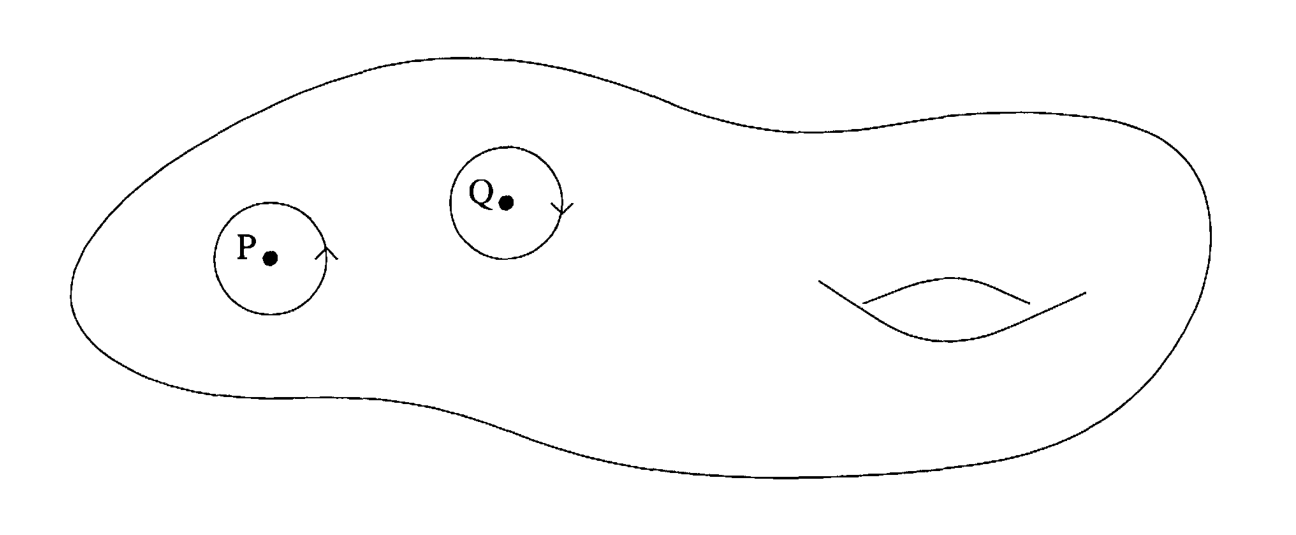
\includegraphics[width=0.62\textwidth]{figs/fig_p112_1.png}
  \caption{带两个穿刺点 $P$、$Q$ 的曲面 $\Sigma$：$P$、$Q$ 各被一个小圆标出，表示 $\tilde\sigma$ 的相位割线（箭头指示绕行方向，绕行一周相位增加 $\pm2\pi$）；右侧的弧线示意 $\Sigma$ 的亏格（把手）。（原文 Figure 1，p.112）}
  \label{fig:p112-1}
\end{figure}

% [Tutor Note: $\tilde\sigma$ 的缠绕数取 $+1,-1$ 由 (8.24) 的归一化决定：$\frac{1}{2\pi}\int_{\text{绕}P\text{的小圆}}d\theta=1$，故 $\frac{1}{2\pi}\oint d\alpha=+1$，即 $\alpha$ 绕 $P$ 一周增加 $2\pi$；绕 $Q$ 时因 $\delta_P-\delta_Q$ 的符号相反而得 $-1$。这也说明 (8.26) 中的 $\theta$ 不能随手扔掉：把它吸收进 $\tilde\sigma$ 之后，$\tilde\sigma$ 已不再是 $\Sigma$ 上的映射，而是 $\Sigma-P-Q$ 上的多值映射，路径积分要在「不能延拓过 $P,Q$ 的映射」这一类上进行。图中 $P$、$Q$ 处的小圈正是这一割线的位置。]

现在有两类算符：一类在其中一个图像中是局部的，另一类在另一个图像中是局部的。算符 $e^{in\phi(P)}$（在第一种描述中）被映到另一种描述中的一条指令：「把 $P$ 从 $\Sigma$ 上删去，并对绕 $P$ 缠绕数为 $n$ 的 $\sigma$ 作路径积分」。反过来，第二种描述中的普通局部算符 $e^{in\sigma}(P)$，在第一种描述中对应一条非局部的处方。

\subsection{三维对偶}
% 原文 §8.3：Duality in three dimensions

现在转向三维理论。先考察一个 $S^1$ 值函数 $\phi$ 在（固定的）紧致三维流形 $M$（可以带边界）上的理论，其拉格朗日量为
\begin{equation}
  \tag{8.27}
  \label{eq:8-27}
  \mathcal{L}=\frac{\Lambda}{4\pi}\int d^3x\,\sqrt{g}\,\partial_\alpha\phi\,\partial^\alpha\phi
  =\frac{\Lambda}{4\pi}\int d\phi\wedge\ast d\phi .
\end{equation}
三维的一个新奇之处是：前因子 $\Lambda$ 具有质量的量纲。由于 $\Lambda$ 是带量纲的量而非常数，在 $\Lambda$ 取某个数值时不可能发生任何特殊的事情。

我们把理论推广到 $\phi$ 是平凡 $S^1$-丛 $\mathcal{L}_B$ 的截面、并带有联络 $B$ 的情形，写下包含协变导数 $D_B\phi=d\phi+B$ 的拉格朗日量：
\begin{equation}
  \tag{8.28}
  \label{eq:8-28}
  \mathcal{L}(\phi,B)=\frac{\Lambda}{4\pi}\int d^3x\,(\partial_\alpha\phi+B_\alpha)(\partial^\alpha\phi+B^\alpha)
  =\frac{\Lambda}{4\pi}\int D_B\phi\wedge\ast D_B\phi
\end{equation}
如果把它当作一个自成体系的理论、把 $B$ 与 $\phi$ 都当作量子场，那么它是一个相当平庸的理论；经典运动方程告诉我们，在差一个规范变换的意义下一切都是零，量子理论同样平庸。为了有所进展，我们引入一个带有联络 $A$ 的线丛 $\mathcal{L}$，以及拉格朗日量
\begin{equation}
  \tag{8.29}
  \label{eq:8-29}
  \mathcal{L}(\phi,B,A)=\frac{\Lambda}{4\pi}\int D_B\phi\wedge\ast D_B\phi-\frac{i}{2\pi}\int A\wedge F_B,
\end{equation}

% ===== 原文 p.113 =====
把最后一项理解为 $-\frac{i}{2\pi}\int F_A\wedge B$（在分部积分之后）；这样做是合理的，因为 $\mathcal{L}_B$ 平凡，而且在给定平凡化之后，$B$ 就只是一个 1-形式。当 $\mathcal{L}_B$ 非平凡时，其推广是路径积分中的一个因子 $e^{\frac{i}{2\pi}\int A\wedge F_B}$，我们把其中的指数解释为丛 $\mathcal{L}\oplus\mathcal{L}_B$ 上联络 $A\oplus B$ 的 Chern–Simons 不变量。这个因子是良定义的，因为 Chern–Simons 不变量给出到 $\mathbb{R}/2\pi\mathbb{Z}$ 的良定义映射。

为了执行对偶变换，我们需要对线丛 $\mathcal{L}$ 求和，从而得到一个路径积分
\begin{equation}
  \tag{8.30}
  \label{eq:8-30}
  \frac{1}{\mathrm{vol}(G)\mathrm{vol}(G')}\sum_{\mathcal{L}}\int\mathcal{D}\phi\,\mathcal{D}A\,\mathcal{D}B\,
  \exp\Bigl[-\frac{\Lambda}{4\pi}\int D_B\phi\wedge\ast D_B\phi+\frac{i}{2\pi}\int F_A\wedge B\Bigr],
\end{equation}
其中 $G$ 与 $G'$ 分别是 $\mathcal{L}$ 与 $\mathcal{L}_B$ 的规范群。

我们想积掉 $A$。粗略的说法是：这样做会给出 $\delta(F_B)$，从而意味着 $B$ 是平坦联络。正如我们在二维所作的计算那样，复杂性来自 $B$ 具有非平凡和乐的可能性。事实上，若 $F_B=0$，我们可以把 $B$ 看作 $H^1(M,\mathbb{R}/\mathbb{Z})$ 的一个元素，并对每个 $x=c_1(\mathcal{L})$ 定义量 $e^{2\int x\wedge[B]}$。当对 $A$ 作路径积分时对 $[x]$ 求和，结果就是 $\delta([B])$，这表明 $B$ 与平凡平坦联络规范等价。于是我们回到原来的理论；我们已经看到，带有 $A$ 与 $\mathcal{L}$ 的扩充理论等价于原来的理论。

现在我们从相反的方向作积分，即作 $\phi$ 与 $A$ 的积分。如同二维情形，我们通过规范变换把 $\phi$ 置零，从而去掉归一化因子 $(\mathrm{vol}(G))^{-1}$。（与二维不同，Faddeev–Popov 行列式不贡献任何有趣的东西，所以我们不显式写出它。）在所得的路径积分中可以配方：
\begin{align}
  \tag{8.31}
  \label{eq:8-31}
  \frac{1}{\mathrm{vol}(G')}\sum_{\mathcal{L}}\int\mathcal{D}A\,\mathcal{D}B\,
  &\exp\Bigl[-\frac{\Lambda}{4\pi}\int B\wedge\ast B+\frac{i}{2\pi}\int B\wedge F_A\Bigr]\\
  \tag{8.32}
  \label{eq:8-32}
  =\frac{1}{\mathrm{vol}(G')}\sum_{\mathcal{L}}\int\mathcal{D}A\,\mathcal{D}B'\,
  &\exp\Bigl[-\frac{\Lambda}{4\pi}\int B'\wedge\ast B'-\frac{1}{4\pi\Lambda}\int F_A\wedge\ast F_A\Bigr],
\end{align}
其中我们作了平移 $B'=B-\frac{i}{\Lambda}\ast F_A$。对 $B'$ 的积分是 Gauss 型的，可以并进路径积分的归一化，于是剩下
\begin{equation}
  \tag{8.33}
  \label{eq:8-33}
  \frac{1}{\mathrm{vol}(G')}\sum_{\mathcal{L}}\int\mathcal{D}A\,\exp\Bigl[-\frac{1}{4\pi\Lambda}\int F_A\wedge\ast F_A\Bigr],
\end{equation}
这正是 Abel 规范理论中那个熟悉的路径积分，规范耦合为 $e=\sqrt{\Lambda}$。

% [Tutor Note: (8.31)→(8.32) 的配方有两处容易漏掉的技术点。其一，三维中 $F_A\wedge F_A$ 是 4-形式，恒等于零，所以配方后不会留下 $\int F\wedge F$ 型拓扑项；若照搬到四维，就会出现 $\frac{\theta}{8\pi^2}\int F\wedge F$ 那样的项，那正是四维 $SL(2,\mathbb{Z})$ 对偶与 $\theta$ 角的来源。其二，$B$ 与 $F_A$ 的缩并要用三维的 $\ast^2=+1$（1-形式、2-形式皆然，与二维 1-形式上的 $\ast^2=-1$ 相反），据此 $B'=B-\frac{i}{\Lambda}\ast F_A$ 才消去交叉项并留下 $-\frac{1}{4\pi\Lambda}\int F_A\wedge\ast F_A$；若符号弄错会得到 $+\frac{1}{4\pi\Lambda}$，与 (8.33) 所要求的正定 $U(1)$ 作用量不符。读者可用同法逐项核对二维 (8.19) 与三维 (8.32) 两处配方的符号。]

现在我们要映射算符。与二维所作类似的计算表明：$d\phi$ 在更大的理论中扩充为协变导数 $D_B\phi=d\phi+B$，而在对偶理论中变为 $\frac{i}{\Lambda}\ast F_A$。这就是 Laplace 方程的解与 Maxwell 方程的解之间的对偶在量子理论中的含义。

那么 $e^{in\phi(P)}$ 这样的算符呢？这个我们不去做，但我会陈述答案：$e^{in\phi(P)}$ 在对偶的规范理论中被映到如下指令：把点 $P$ 从三维流形 $M$ 上删去，并考虑线丛 $\mathcal{L}$ 上联络的路径积分，其中 $\mathcal{L}$ 的第一 Chern 类在一个小

% ===== 原文 p.114 =====
球面（围绕 $P$）上取值 $n$。导致这一点的论证与我们在二维所做的基本一致。

我不打算给出那个论证（我把它推荐为一道练习），而是讨论大致相反的方向。我们考虑规范理论中的 Wilson 圈（Wilson loop）算符，并试着把它们映回标量场论。

设 $C$ 是 $M$ 中一个作为边界的圆，$\lambda\in\mathbb{R}$。规范理论中有算符 $\exp(i\lambda\oint_C A)$。我们把它插入大理论（即拉格朗日量为 $\mathcal{L}(\phi,B,A)$ 的那个理论）的路径积分。（更一般地，即使 $C$ 不是边界我们也可以这样做，但那时 $\lambda$ 必须限制为整数。设 $C$ 是某个二维曲面 $D$ 的边界，则可写 $\exp(i\lambda\oint_C A)=\exp(i\lambda\int_D F)$，这表明对任意 $\lambda$ 都规范不变。）

当我们在路径积分中带上这个额外因子去积掉 $A$ 时，得到的不是 $\delta(F_B=0)$，而是 $\delta(F_B=2\pi\lambda[C])$，其中 $[C]$ 是 $C$ 的 Poincaré 对偶。换言之，作 $A$ 积分把 $B$ 确定为满足 $F_B=2\pi\lambda[C]$，而积掉 $A$ 之后修改过的拉格朗日量是 $\int D_B\phi\wedge\ast D_B\phi$。这里 $B$ 是平坦的 $U(1)$ 联络，绕该圆有单值性（monodromy）$e^{2\pi i\lambda}$。于是，圆 $C$ 上的 Wilson 圈算符对偶于如下处方：「删去 $C$，并把 $\phi$ 解释为平坦圆丛的一个截面，其绕 $C$ 的加法单值性为 $2\pi\lambda$。」换句话说，我们修改 $\phi$ 为 $\tilde\phi$，使得 $d\tilde\phi=d\phi+B$，并把 $\tilde\phi$ 解释为 $M-C$ 上平凡 $S^1$-丛的一个截面，带有绕 $C$ 的单值性为 $e^{2\pi i\lambda}$ 的平坦联络。（要得到这样一个平凡 $S^1$-丛，我们或者需要假定 $C$ 是边界，或者需要 $\lambda$ 是整数。一切都自洽，因为这些也正是我们出发时的 Wilson 线为规范不变的条件。）

% [Tutor Note: $\delta(F_B=2\pi\lambda[C])$ 中的 $2\pi$ 必须与 (8.29) 的 $\frac{i}{2\pi}\int A\wedge F_B$ 的归一化配套：插入 $e^{i\lambda\oint A}=e^{i\lambda\int_D F}$ 相当于给 $A$ 的线性项加上 $i\lambda\int A\wedge\cdots$，对 $A$ 变分即得 $F_B=2\pi\lambda[C]$，于是 $\oint_C B=2\pi\lambda$、单值性为 $e^{2\pi i\lambda}$。若 $C$ 不是边界而 $\lambda\notin\mathbb{Z}$，$\oint A$ 本身无定义（须先取平凡化），这就是作者强调「$C$ 是边界、或 $\lambda$ 为整数」的原因——它也是 Dirac 量子化条件在三维的翻版：磁单极子（此处即 $A$ 的第一 Chern 类非零的构型）的荷必须量子化。]

\subsection{应用于 Polyakov 模型}
% 原文 §8.4：Application to the Polyakov model

我们将描述一个 Polyakov 大约在 1975 年构造的模型。这是对偶在一个非线性相对论性理论中的首次使用。该模型展示了被称为禁闭的现象。

我们在三维工作，研究带有标量场 $s$（属于三维表示）的 $SO(3)$ 规范理论，其拉格朗日量为
\begin{equation}
  \tag{8.34}
  \label{eq:8-34}
  \mathcal{L}=\frac{1}{4\pi e^2}\int d^3x\,\mathrm{Tr}\,|F|^2
  +\int d^3x\,(D\vec s)^2+\int d^3x\,\lambda(\vec s^{\,2}-a^2)^2 .
\end{equation}
这个模型在树图阶（tree level）展示了 Higgs 机制。

经典地，通过一个规范变换可以把真空转到
\begin{equation}
  \tag{8.35}
  \label{eq:8-35}
  \langle\vec s\rangle=\begin{pmatrix}a<本地路径>
\end{equation}
在真空态中，拉格朗日量的 $SO(3)$ 对称性破缺为 $SO(2)=U(1)$ 对称性，唯一的无质量场是 $U(1)$ 联络。（这就是所谓的 Higgs 机制。）低能理论看起来就像三维的 $U(1)$ 理论。

\textbf{第一步（First Step）.} 在低能下，这个理论经典地看起来像拉格朗日量为
\begin{equation}
  \tag{8.36}
  \label{eq:8-36}
  \mathcal{L}=\frac{1}{4e^2}\int F\wedge\ast F
\end{equation}
的 $U(1)$ 规范理论。

这就是答案吗？自由 $U(1)$ 理论的高斯不动点（Gaussian fixed point）稳定吗？

% [Tutor Note: 对照 (8.34) 与 (8.36)：前者为 $\frac{1}{4\pi e^2}\int\mathrm{Tr}|F|^2$，后者为 $\frac{1}{4e^2}\int F\wedge\ast F$，两处系数相差一个 $\pi$。这不一定是笔误——$\mathrm{Tr}$ 在伴随表示上的归一化、以及 $F\wedge\ast F=|F|^2d^3x$ 的约定都可以吸收常数——但读者若要把 (8.36) 的低能有效耦合与 (8.34) 的树图耦合直接比较（例如估算 Higgs 机制给出的规范场质量 $m\sim ea$ 与低能耦合 $e$ 的关系），必须先统一两处的归一化，否则会整体差出 $\sqrt{\pi}$。]
